\documentclass{article}

% Packages
\usepackage[a4paper, total={210mm, 297mm}, includehead, includefoot,margin=2.5cm]{geometry}
\usepackage[english]{babel}
\usepackage{comment}
\usepackage{xcolor}
\usepackage{amsmath, amsfonts, amssymb}
\usepackage{float}
\usepackage{graphicx}
\usepackage{fancyhdr}
\usepackage{lastpage}
\usepackage{hyperref}
\usepackage{pagecolor}
\usepackage{mdframed}
\usepackage{lipsum}
\usepackage{url}
\usepackage{parskip}
\usepackage{mathtools}
\usepackage{centernot}
\usepackage[most]{tcolorbox}


\usepackage{tikz}
\usetikzlibrary{arrows,decorations.markings}
\usetikzlibrary{matrix, positioning, fit}




% Settings
\hypersetup{colorlinks=true,linkcolor=black,filecolor=magenta,urlcolor=cyan}
\urlstyle{same}

\newcommand*{\QEDA}{\hfill\ensuremath{\blacksquare}}
\newcounter{pic}[page]
\newcounter{fig}[page]
\numberwithin{equation}{section}

\newmdtheoremenv[
	linecolor=IdealColour,
	leftmargin=0,
	rightmargin=0,
	outerlinecolor=IdealColour,
	outerlinewidth=2,
	roundcorner=60pt,
	backgroundcolor=white,
	innertopmargin=10pt,
]{diagram}{Diagram}[section]

\newmdtheoremenv[
	linecolor=IdealColour,
	outerlinecolor=IdealColour,
	outerlinewidth=2,
	roundcorner=60pt,
	backgroundcolor=LightGray,
	innertopmargin=10pt,
]{principle}{Principle}[section]

% Colours
\usepackage{xcolor}
\definecolor{HeadColour}{HTML}{376092}
\definecolor{IdealColour}{HTML}{ff6e6e}
\definecolor{LightGray}{gray}{0.9}
\renewcommand{\footrulewidth}{0.4pt}
\renewcommand{\baselinestretch}{1.5}

\pagestyle{fancy}
\fancyhead{}
\fancyfoot{}
\fancyhead[L]{\textbf{\textsc{IDEal}.}}
\fancyhead[R]{\today}
\fancyfoot[R]{Page \thepage \hspace{1pt} of \pageref*{LastPage}}

% Custom Commands
\newcommand{\ft}[1]{\mathcal{F}\{#1\}}
\newcommand{\Laplace}[1]{\ensuremath{\mathcal{L}{\left[#1\right]}}}
\newcommand{\InvLap}[1]{\ensuremath{\mathcal{L}^{-1}{\left[#1\right]}}}
\newcounter{NumberInTable}
\newcommand{\LTNUM}{\stepcounter{NumberInTable}{(\theNumberInTable)}}

\newcommand{\ideal}{\textsc{IDEal }}
\newcommand{\braket}[1]{\langle #1 \rangle}
\newcommand{\objectas}[2]{$\braket{#1 \ \text{as} \ #2}$}

\newcommand{\quickexample}[1]{
\begin{tcolorbox}[%
    enhanced, 
    breakable,
    frame hidden,
    overlay broken = {
	\draw[line width=0.01mm, black, rounded corners] (frame.north west) rectangle (frame.south east);
},
    ]{}
	\textbf{Example.} #1
\end{tcolorbox}
}

% Title
\date{\today}

\begin{document}

	\pagecolor{IdealColour}

	\begin{titlepage}
	\begin{center}
		\color{white}
		\vfill
		\line(1,0){400}\\[1mm]
			\huge{\textbf{IDEal: A Legal Development Environment}}\\
			\Large{\textbf{Australian Submission}}\\
			2020 \\
		\line(1,0){400}\\[3mm]
		\vfill
		\large{Mamta Thaker | Joanna Chen | Mirhady Dorodjatun | Joshua Fourie}
	\end{center}
	\end{titlepage}

	\pagecolor{white}

	\tableofcontents
	\thispagestyle{empty}
	\clearpage

%----------------------------------- TECHNICAL PART -------------------------------------%

\pagebreak
\part{Theory}

A legal matter processed in \ideal traverses four states:
\begin{itemize}
	\item \textit{Generation} ($\mathcal{G}$). 
	\item \textit{Representation} ($\mathcal{R}$).
	\item \textit{Transformation} ($\mathcal{T}$). 
	\item \textit{Presentation} ($\mathcal{P}$).
\end{itemize}
	
We can understand \ideal as a system of \textit{plug-ins} which either generate, or commonly access and transform a unified representation of a legal matter into derivative states. Consequently, the system is a series of machines mapping $[ \ \alpha_i \in \mathcal{G \cup T \cup P} \ ] \rightarrow \mathcal{R}$, or $\mathcal{R} \rightarrow [ \ \beta_i \in \mathcal{G \cup T \cup P} \ ]$. We denote $\braket{\alpha_i}$ as a \textit{generator} state which can generate $\mathcal{R}$, and $\beta_i$ as a \textit{producible} state, which can be produced by some action on $\mathcal{R}$.
\begin{figure}[h]
\begin{center}
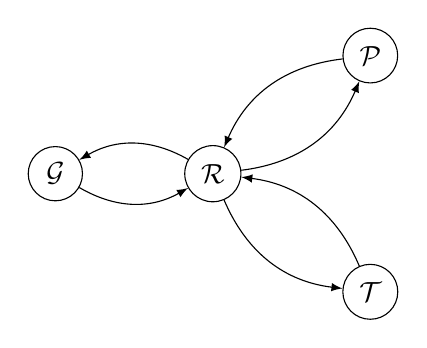
\begin{tikzpicture}
	\node[shape=circle, draw=black] (G) at (-2, 0) {$\mathcal{G}$};
	\node[shape=circle, draw=black] (R) at (0, 0) {$\mathcal{R}$};
	\node[shape=circle, draw=black] (T) at (2, -1.5) {$\mathcal{T}$};
	\node[shape=circle, draw=black] (P) at (2, 1.5) {$\mathcal{P}$};


	\path[->, >=latex] (G) edge[bend right] node {} (R);
	\path[->, >=latex] (R) edge[bend right] node {} (G);

	\path[->, >=latex] (R) edge[bend right] node {} (T);
	\path[->, >=latex] (T) edge[bend right] node {} (R);

	
	\path[->, >=latex] (R) edge[bend right] node {} (P);
	\path[->, >=latex] (P) edge[bend right] node {} (R);
	
\end{tikzpicture}
\end{center}
\caption{Visualising the interactions between the states.}
\end{figure}

%---------------------- DEFINING THE REPRESENTATION -------------------------------%

\section{Defining the Representation}

Our goal is to define a mathematical structure for $\mathcal{R}$ which encodes legal information and maximises the number of producible states. Given that the representation is driven by the encoded legal information, we begin with the idea that a lawyer is a mechanism for analysing the \textit{existence} or \textit{non-existence} of a legal relationship between \textit{objects}. 

%------------------------- Nodes and NodeState ----------------------------%

\paragraph{Facts, Nodes and the NodeState.} We describe a legal object as a \texttt{Node}, and define the admissible \textit{factual} actions, attributes or character of the \texttt{Node} as the \texttt{NodeState}. The $\texttt{NodeState}_n$ is an unordered set of $n$  \texttt{Fact} objects which are generated and edited by an oracle, $\mathcal{F}$, in combination with a \texttt{SourceOfLaw}: % In the below, does a set of n always imply a nodestate of n?
\begin{align}
	\mathcal{F}: (\texttt{SourceOfLaw}, \ \{ \ \texttt{Fact}_0, .., \ \texttt{Fact}_n \ \}) \rightarrow \texttt{NodeState}_n \\
	\mathcal{F}: (\texttt{Fact}, \ \texttt{NodeState}_n) \rightarrow \texttt{NodeState}_{n'} \\
	\mathcal{F}: \texttt{NodeState}_n \rightarrow \texttt{NodeState}_{n''}
\end{align}

\paragraph{Sources of Law.} A \texttt{SourceOfLaw} defines the conditions, attributes or characteristics which are required for the oracle to generate both a \texttt{NodeState}, as well as the \texttt{Role} (\ref{section:role-object}) associated with a \texttt{NodeState}. Concretely, these are objects such as legislation or common law which have the inherent capacity to generate legal rights or obligations relevant to an object.

%--------------------------------- ROLE -----------------------------------------%

\subsection{The Role Object} \label{section:role-object}

A \texttt{Role} defines the \textit{legal personality} of a \texttt{Node} by capturing the attributes, actions, or characterstics attributable under law. A \texttt{Node} can be subject to multiple \texttt{Role} objects of arbitrary complexity, provided they are distinct under (\ref{eq:role-equivalence}). The \texttt{Role} associated with a \texttt{Node} is generated by a pair \texttt{(NodeState, SourceOfLaw)} under the oracle function, $\mathcal{F}$, and is transformable under the \texttt{Consequence} of a \texttt{Link} (\ref{section:links}): 
\begin{align}	
	\mathcal{F} : [ \ \texttt{(NodeState, SourceOfLaw)} \rightarrow \texttt{Role} \ ] \\
	\texttt{Consequence} : [ \ \texttt{Role} \rightarrow \texttt{Role'} \ ]
\end{align}

\paragraph{Equivalence of Roles.} We define an equivalence relation on a pair $(\texttt{Role}_i, \ \texttt{Role}_j)$ by comparing their generating states, such that they are only pairwise distinct where the generative facts and law diverge:  
\begin{equation}\label{eq:role-equivalence}
[ \ \texttt{Role}_i = \texttt{Role}_j \ ] \iff [ \ (\texttt{NodeState}_i \iff \texttt{NodeState}_j) \land (\texttt{SourceOfLaw}_i \iff \texttt{SourceOfLaw}_j) \ ]
\end{equation}

\paragraph{Role Extension.} The \texttt{NodeState} of a \texttt{Node} can generate multiple \texttt{Role} objects \textit{iff} the (\texttt{NodeState, SourceOfLaw}) pair are distinct under (\ref{eq:role-equivalence}). A \texttt{Role} is \textit{reducible} when a subset of the generative \texttt{NodeState} can produce another distinct \texttt{Role}:
\begin{align}
	[ \ N := \{ \texttt{Fact}_0, .., \texttt{Fact}_n \} \ ] \land [ \ M := \{ \texttt{Fact}_0, .., \texttt{Fact}_m \} \ ] : [ \ M \subset N \ ] \\
	[ \ \texttt{NodeState}_i = \mathcal{F}(N, \texttt{SourceOfLaw}_i) \ ] : \ [ \ \texttt{Role}_i = \mathcal{F}(\texttt{NodeState}_i, \ , \texttt{SourceOfLaw}_{i'}) \ ] \\
	[ \ \texttt{NodeState}_j = \mathcal{F}(M, \texttt{SourceOfLaw}_j) \ ] : \ [ \ \texttt{Role}_j = \mathcal{F}(\texttt{NodeState}_j, \texttt{SourceOfLaw}_{j'}) \ ] \\
	\qquad \implies [ \ \texttt{$N$ is \textit{reducible}} \ ]
\end{align}

A \texttt{Role} which is reducible is an \textit{extension} of another \texttt{Role}, and the \texttt{Role} objects which are extended are called the \textit{components of the extension}. The extended \texttt{Role} will automatically import any components of the extension objects into its own definition. We denote an extension using subset notation, such that the following indicates $\texttt{Role}_i$ is an extension of $\texttt{Role}_j$: 
\begin{align}
	\texttt{Role}_j \subset \texttt{Role}_i \\
	[ \ \texttt{Role}_j \subset \texttt{Role}_i \ ] : [ \ \texttt{Role}_i \implies \texttt{Role}_j \ ]
\end{align}

Given that an extension implies any components of the extension, a \texttt{Node} with multiple \texttt{Role} objects \textit{may} replace any \texttt{Role} with an extension. We distinguish a \texttt{Role} extension from a \texttt{Role} \textit{composition}, which is a set of distinct \texttt{Role} objects where there does not exist a \texttt{Role} in the composition which is an extension of any other \texttt{Role}:
\begin{align}
	[ \ N := \ \{ \ \texttt{Role}_0, .., \texttt{Role}_n \ \} \ ] : [ \ \nexists (\texttt{Role}_i, \texttt{Role}_j) \in N : \texttt{Role}_i \subset \texttt{Role}_j \ ]
\end{align}

% TODO: Incorporate? : Furthermore, whilst an automorphic \texttt{Link} over an irreducible \texttt{Role} is undefined behaviour, an extension can freely modify any components.

%---------------------------- LINKS AND CONSEQUENCES ---------------------------------%

\subsection{Links}\label{section:links}

A \texttt{Link} is a directed, pairwise relationship between a source ($\texttt{Role}_i$) and a destination ($\texttt{Role}_j$), which has been generated with the assistance of a \texttt{SourceOfLaw}. Given a pair $(\texttt{Role}_i, \texttt{Role}_j)$ and an associated \texttt{SourceOfLaw}, the oracle may draw a $\texttt{Link}_{i \rightarrow j}$:
\begin{align}
	\mathcal{F} : (\texttt{SourceOfLaw}, \ \texttt{Role}_i, \ \texttt{Role}_j) \rightarrow  \texttt{Link}_{i \rightarrow j}
\end{align}

\paragraph{Hooking a Link.} The \texttt{Hook} and \texttt{Anchor} objects are a specialisation of the \texttt{Role} object which represent the directed, relational requirements of a \texttt{Link}, and are generated under a (\texttt{SourceOfLaw, Role}) pairing. The oracle defines a \texttt{Link} by consuming a (\texttt{SourceOfLaw}, \texttt{Hook}, \texttt{Anchor}) triple:
\begin{align}
	[ \ \mathcal{F}(\texttt{SourceOfLaw}, \ \texttt{Role}_i) = \texttt{Hook} \ ] \ \land \ [ \ \mathcal{F}(\texttt{SourceOfLaw}, \ \texttt{Role}_j) = \texttt{Anchor} \ ] \\
	\implies \mathcal{F}: (\texttt{SourceOfLaw}, \ \texttt{Role}_i, \ \texttt{Role}_j) \rightarrow (\texttt{Hook, Anchor}) \\ 
	\mathcal{F} : (\texttt{SourceOfLaw, Hook, Anchor}) \rightarrow \texttt{Link}_{i \rightarrow j}
\end{align}

\subsection{Consequence} 

Given a \texttt{Link} to a relationship, the oracle, $\mathcal{F}$, generates a \texttt{Consequence} from a \texttt{SourceOfLaw}:
\begin{equation}
	\texttt{Link}_{i \rightarrow j} \implies [ \ \mathcal{F} : \texttt{SourceOfLaw} \rightarrow \texttt{Consequence} \ ]
\end{equation}

A \texttt{Node} may be modified under the \texttt{Consequence} of a \texttt{Link}, changing the \texttt{NodeState} or associated \texttt{Role}: 
\begin{equation}
	[ \ \mathcal{F}(\texttt{Consequence, Node}) = \texttt{Node'} \ ] \implies \{ \ [ \ \texttt{NodeState} \rightarrow \texttt{NodeState'} \ ] \lor [ \ \texttt{Role}_i \rightarrow \texttt{Role}_i' \ ] \ \}
\end{equation}

The oracle subsequently \textit{walks the consequence forward} to generate or decouple any \texttt{Hook} or \texttt{Anchor} objects which have been invalidated by a disturbance of the \texttt{Conditions} required by the \texttt{SourceOfLaw}.

\subsection{Sources of Law}
Given a \texttt{SourceOfLaw}, there exists a related set of \texttt{Conditions} which must be satisfied before the oracle function, $\mathcal{F}$, can evaluate any expression:
\begin{align}
	\texttt{SourceOfLaw} \implies \texttt{Conditions} \\
	\mathcal{F} : \texttt{Conditions} \rightarrow \{ \ T, F \ \}
\end{align}

\paragraph{Application to Links.} The \texttt{Hook} or \texttt{Anchor} required to draw a \texttt{Link} will have \texttt{Conditions} containing evaluations related to the \texttt{NodeState} of an object. The oracle, $\mathcal{F}$, will only generate a \texttt{Link} where the \texttt{Conditions} imposed by the \texttt{SourceOfLaw} are satisfied. Consequently, a \texttt{Link} will 'decouple' where a \texttt{Consequence} modifies the \texttt{NodeState} such that the evaluation of the \texttt{Conditions} of the relevant \texttt{SourceOfLaw} fail.


%------------------------ Stage ---------------------------------%

% there's some tension around a consequence: should it progress the stage controller?

\subsection{The Stage Controller}

\textit{Time} is encoded in $\mathcal{R}$ as an ordered set of $n$ distinct \texttt{Interval} objects related by a \texttt{Transition}:
\begin{align}
	\texttt{IntervalSet} := \ \{ \ \texttt{Interval}_0, .., \texttt{Interval}_n \ \} \\
	\texttt{ForwardTransition} : \texttt{Interval}_i \rightarrow \texttt{Interval}_{i + 1}\\
	\texttt{BackwardTransition} : \texttt{Interval}_i \rightarrow \texttt{Interval}_{i - 1}
\end{align}

The \texttt{BackwardTransition} and \texttt{ForwardTransition} are a specialisation of a \texttt{Transition} that form an identity map under function composition:
\begin{align}
	\texttt{BackwardTransition} \circ \texttt{ForwardTransition} : a \rightarrow a
\end{align}

The \texttt{TransitionSet} of an \texttt{Interval} is the minimum set of \texttt{ForwardTransition} and \texttt{BackwardTransition} objects required to reconstruct the \texttt{IntervalSet} under the oracle function, $F$:
\begin{align}
	\mathcal{F}: (\texttt{TransitionSet}, \texttt{Interval}) \rightarrow  \texttt{IntervalSet}
\end{align}


\vspace{0.25cm}
\quickexample{

Consider a boundary dispute between $\mathcal{A}lice$ and $\mathcal{B}ob$ on two adjacent plots of land: $\mathcal{L}_a$ and $\mathcal{L}_b$. In this case, $\mathcal{A}lice$ is the owner of $\mathcal{L}_a$, and $\mathcal{B}ob$ is the owner of $\mathcal{L}_b$. We are attempting to define whether it is permissible for $\mathcal{A}lice$ to build a structure by defining a boundary line delineating the properties, called \texttt{Bound}. The graphs below represents the information encoded in $\texttt{Interval}_0$.

\begin{diagram}{$\mathcal{A}lice$ owns a parcel of land. \\ }
\begin{minipage}{0.45\textwidth}
\vspace{0.25cm}
\begin{tikzpicture}[font=\ttfamily,
  bigContainer/.style={matrix of nodes, nodes=typetag, row sep=1em},
  smallContainer/.style={draw=gray, inner sep=1ex},  
  typetag/.style={draw=gray, inner sep=1ex, anchor=west},
  title/.style={draw=none, color=gray, inner sep=0pt}
]
%----------- A_PERSON:	

	%---------- BOX AROUND A_PERSON 
	\coordinate (A1) at (-3, 3);
	\coordinate (A2) at (0, 3);
	\coordinate (A3) at (0, -1);
	\coordinate (A4a) at (-3, -1);
	\coordinate (A4b) at (-3, 0.5);
	\coordinate (A4c) at (-3, 1.5);
	\draw[-, dotted] (A1) -- (A2);
	\draw[-, dotted] (A2) -- (A3);
	\draw[-, dotted] (A3) -- (A4a);
	\draw[-, dotted] (A4a) -- (A4b);	
	\draw[-, dotted] (A4c) -- (A1);
	
	%---------- NODES WITHIN A_PERSON 
	\node[shape=rectangle, color=gray] (A) at (-1.5, 2.75) {$\mathcal{A}lice$};
	\node[shape=rectangle, draw=black] (A_State) at (-1.5, 2) {Purchased $\mathcal{L}_a$};
	\node[shape=rectangle, draw=blue] (A_Law) at (-4.5, 1) {Property Act: sX.X};
	\node[shape=rectangle, draw=red] (A_Role) at (-1.5, -0.5) {Owner of $\mathcal{L}_a$};
	
	%---------- LINES BETWEEN NODES WITHIN A_PERSON 
	\node[shape=circle, draw=black] (A5) at (-1.5, 1) {$+$};
	\draw[-] (A_Law) -- (A5);
	\draw[-] (A_State) -- (A5);
	\draw[->] (A5) -- (A_Role);

%---------- A_LAND:

	%---------- BOX AROUND A_LAND
	\coordinate (B1) at (1.5, 3);
	\coordinate (B2a) at (4.5, 3);
	\coordinate (B2b) at (4.5, 1.5);
	\coordinate (B2c) at (4.5, 0.5);
	\coordinate (B3) at (4.5, -1);
	\coordinate (B4) at (1.5, -1);
	\draw[-, dotted] (B1) -- (B2a);
	\draw[-, dotted] (B2a) -- (B2b);
	\draw[-, dotted] (B2c) -- (B3);
	\draw[-, dotted] (B3) -- (B4);	
	\draw[-, dotted] (B4) -- (B1);

	%---------- NODES WITHIN A_LAND 
	\node[shape=rectangle, color=gray] (B) at (3, 2.75) {$\mathcal{L}_a$};
	\node[shape=rectangle, draw=black] (B_State) at (3, 2) {$\mathcal{L}_a$ is land};
	\node[shape=rectangle, draw=blue] (B_Law) at (6, 1) {Property Act: sY.Y};
	\node[shape=rectangle, draw=red] (B_Role) at (3, -0.5) {Land };

	%---------- LINES BETWEEN NODES WITHIN A_LAND 
	\node[shape=circle, draw=black] (B5) at (3, 1) {$+$};
	\draw[-] (B_Law) -- (B5);
	\draw[-] (B_State) -- (B5);
	\draw[->] (B5) -- (B_Role);
	
%--------- LINK A_PERSON -> A_LAND:
	\coordinate (A_Person_Hook_End) at (3.1, -2);

	\node[draw=blue, shape=rectangle] (A_B_Law) at (-4.5, -2) {Property Act: sZ.Z};
	\node[draw=black, shape=circle] (A_B_Law_Link) at (-1.5, -2) {$+$};
	\node[draw=gray, shape=circle, scale=0.06] (A_Person_Anchor) at (3, -1.5)  {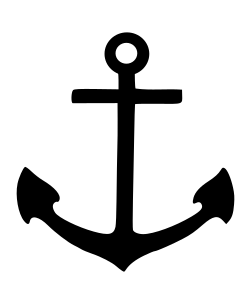
\includegraphics{image/anchor.png}};
	\node[draw=gray] (A_B_Link) at (0.75, -2) {$Owns$};
	
	\draw[-] (A_B_Law) -- (A_B_Law_Link);
	\draw[-] (A_Role) -- (A_B_Law_Link);
	\draw[-] (A_B_Law_Link) -- (A_B_Link);
	\draw[left hook-] (A_Person_Hook_End) -- (A_B_Link);
	\draw[-] (A_Person_Anchor) -- (B_Role);

\end{tikzpicture}
\end{minipage}
\end{diagram}

% TODO: The diagram allows a NodeState without a relevant SourceOfLaw...
% TODO: The diagram allows an anchor without a relevant SourceOfLaw...
The above diagram (\textbf{1.1}) reflects the following:
\begin{enumerate}
	\item $\mathcal{A}lice$ and $\mathcal{L}_a$ are both a \texttt{Node}.
	\item $[ \ Purchased \ \mathcal{L}_a \ ]$ and $[ \ \mathcal{L}_a \ is \ land \ ]$ are both instances of a \texttt{Fact}.
	\item $( \ Property \ Act: \ sX.X, \ Purchased \ \mathcal{L}_a \ )$ generates the \texttt{Role} $[ \ Owner \ of \ \mathcal{L}_a \ ]$.
	\item $( \ Property \ Act: \ sY.Y, \ \mathcal{L}_a \ is \ land \ )$ generates the \texttt{Role} $[ \ Real \ Property \ ]$.
	\item The (\texttt{Hook}, \texttt{Anchor}) pairing below generates a \texttt{Link} $[ \ Owns \ ]$:
	\begin{enumerate}
		\item $( \ Property \ Act: \ sZ.Z, \ Owner \ of \ \mathcal{L}_a \ )$ generates a \texttt{Hook}.
		\item $[ \ Real \ Property \ ]$ generates an \texttt{Anchor}.
	\end{enumerate}
\end{enumerate}

\vspace{0.25cm}

The \texttt{Consequence} of the \texttt{Link} $[ \ Owns \ ]$ requires that any other \texttt{Anchor} on $\mathcal{L}_a$ satisfies the additional \texttt{Condition} of having either a superior 'property' claim in relation to $\mathcal{L}_a$, or $\mathcal{A}lice$'s consent. 

\begin{diagram}{Can $\mathcal{E}ve$ walk on $\mathcal{L}_a$? \\ }
\begin{minipage}{0.45\textwidth}
\vspace{0.25cm}
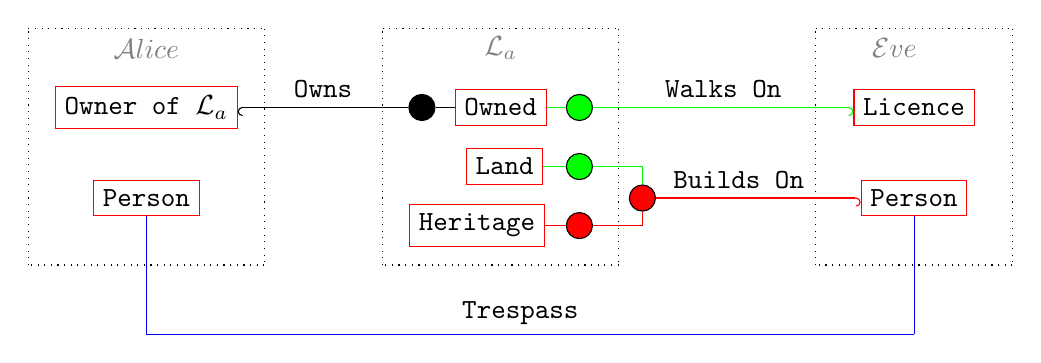
\begin{tikzpicture}[font=\ttfamily,
  bigContainer/.style={matrix of nodes, nodes=typetag, row sep=1em},
  smallContainer/.style={draw=gray, inner sep=1ex},  
  typetag/.style={draw=gray, inner sep=1ex, anchor=west},
  title/.style={draw=none, color=gray, inner sep=0pt}
]
%------------- Land
	\coordinate (L1) at (1.5, 3);
	\coordinate (L2) at (4.5, 3);
	\coordinate (L3) at (4.5, 0);
	\coordinate (L4) at (1.5, 0);
	\draw[-, dotted] (L1) -- (L2);
	\draw[-, dotted] (L2) -- (L3);
	\draw[-, dotted] (L3) -- (L4);	
	\draw[-, dotted] (L4) -- (L1);


	\node[shape=rectangle, color=gray] (L) at (3, 2.75) {$\mathcal{L}_a$};
	\node[shape=rectangle, draw=red] (L_Owned) at (3, 2) {Owned};
	\node[shape=rectangle, draw=red] (L_Land) at (3.05, 1.25) {Land};
	\node[shape=rectangle, draw=red] (L_Heritage) at (2.7, 0.5) {Heritage};

	\node[draw=black, shape=circle, fill=black] (L_Owned_Consequence) at (2, 2) {};

	\node[draw=black, shape=circle, fill=green] (L_Owned_Condition) at (4, 2) {};
	\node[draw=black, shape=circle, fill=green] (L_Land_Condition) at (4, 1.25) {};
	\node[draw=black, shape=circle, fill=red] (L_Heritage_Condition) at (4, 0.5)  {};
	\node[draw=black, shape=circle, fill=red] (L_Builds_On_Condition) at (4.8, 0.85) {};

	\draw[draw=green] (L_Owned_Condition) -- (L_Owned);
	\draw[draw=green] (L_Land_Condition) -- (L_Land);
	\draw[draw=red] (L_Heritage_Condition) -- (L_Heritage); 
	\draw[draw=green] (L_Land_Condition) -| (L_Builds_On_Condition);
	\draw[draw=red] (L_Heritage_Condition) -| (L_Builds_On_Condition);	

	\draw[draw=black] (L_Owned_Consequence) -- (L_Owned);

%------------- Alice
	\coordinate (A1) at (-3, 3);
	\coordinate (A2) at (0, 3);
	\coordinate (A3) at (0, 0);
	\coordinate (A4) at (-3, 0);

	\draw[-, dotted] (A1) -- (A2);	
	\draw[-, dotted] (A2) -- (A3);
	\draw[-, dotted] (A3) -- (A4);
	\draw[-, dotted] (A4) -- (A1);
	
	\node[shape=rectangle, color=gray] (A) at (-1.5, 2.75) {$\mathcal{A}lice$};
	\node[shape=rectangle, draw=red] (A_Role) at (-1.5, 2) {Owner of $\mathcal{L}_a$};
	\node[shape=rectangle, draw=red] (A_Person) at (-1.5, 0.85) {Person};

	\path[left hook-, draw=black] (A_Role) -- node [above] {Owns} (L_Owned_Consequence);

%-------------- Eve
	\coordinate (E1) at (7, 3);
	\coordinate (E2) at (9.5, 3);
	\coordinate (E3) at (9.5, 0);
	\coordinate (E4) at (7, 0);

	\draw[-, dotted] (E1) -- (E2);	
	\draw[-, dotted] (E2) -- (E3);
	\draw[-, dotted] (E3) -- (E4);
	\draw[-, dotted] (E4) -- (E1);

	\node[shape=rectangle, color=gray] (E) at (8, 2.75) {$\mathcal{E}ve$};
	\node[shape=rectangle, draw=red] (E_Licence) at (8.25, 2) {Licence};	
	\node[shape=rectangle, draw=red] (E_Person) at (8.25, 0.85) {Person};

	\path[right hook-, draw=green] (E_Licence) -- node [above] {Walks On} (L_Owned_Condition);
	\path[right hook-, draw=red] (E_Person) -- node [left=0.25, above] {Builds On} (L_Builds_On_Condition);

	\coordinate[below=1.5 of E_Person] (E_Person_Below); 
	\path[draw=blue] (A_Person) |- (E_Person_Below) node [left=5, above] {Trespass} (E_Person_Below) -- (E_Person);

\end{tikzpicture}
\end{minipage}
\end{diagram}

Diagram (\textbf{1.2}) reflects that:
\begin{enumerate}
	\item $\mathcal{L}_a$ has the \texttt{NodeState} $[ \ Owned \ ]$.
	\item The \texttt{NodeState} $[ \ Owned \ ]$ is a \texttt{Consequence} under the \texttt{Link} $[ \ Owns \ ]$.
	\item The \texttt{Condition} of $[ \ Owns \ ]$ requires that any other \texttt{Anchor} on $\mathcal{L}_a$ has the \texttt{Role} $[ \ Licence \ ]$:
\begin{enumerate}
	\item $\mathcal{E}ve$ may walk on $\mathcal{L}_a$ because:
	\begin{enumerate}
		\item The $[ \ Licence \ ]$ is a \texttt{Hook} which satisfies the \texttt{Conditions} for $[ \ Walks \ On \ ]$.
		\item $[ \ Owned \ ]$ is an \texttt{Anchor} which satisfies the \texttt{Conditions} for \texttt{Link} $[ \ Walks \ On \ ]$.
	\end{enumerate}

	\item $\mathcal{E}ve$ may \textbf{not} build on $\mathcal{L}_a$ because: 
	\begin{enumerate}
	\item $[ \ Person \ ]$ is a \texttt{Hook} which \textbf{does not} satisfy the \texttt{Conditions} for $[ \ Builds \ On \ ]$.
	\item $[ \ Land \ ]$  is an \texttt{Anchor} which satisfies the \texttt{Conditions} for $[ \ Builds \ On \ ]$.
	\item $[ \ Heritage \ ]$  is an \texttt{Anchor} which \textbf{does not} satisfy the \texttt{Conditions} for $[ \ Builds \ On \ ]$.
	\end{enumerate}
\end{enumerate}

\end{enumerate}

}

\pagebreak
%%%%%%%%%%%%%%%%%%%%%%%%%%%%%%% DRAFT %%%%%%%%%%%%%%%%%%%%%%%%%%%%%

\paragraph{Compliance and Deviation.} A lawyer constructs a \texttt{Link(Consequence)} by analysing the \texttt{Role} of an object relative to a set of legal conditions. We define both compliance and deviation as:
\begin{equation}
[ \ \exists \ \texttt{Link(Existence, Consequence)} \ ] \land 
	\begin{cases}
		[ \ \texttt{Role} \implies \texttt{Link(..)} \ ], & \text{Compliance} \\
		[ \ \texttt{Role} \centernot\implies \texttt{Link(..)} \ ], & \text{Deviation}
	\end{cases}
\end{equation}

\vspace{0.25cm}
\quickexample{
	Continuing the previous example, we define compliance as Bob enforcing the terms of C against Alice, because Alice fulfils the relevant \texttt{Role}. Bob could not, however, enforce C against a third party, unless they also fulfilled a role which generated a \texttt{Link} to C.
}


% TODO: Actions progress Time?
% TODO: NULL value to over-ride when a source of law can't be found???
% TODO: Indeterminate..? 'we don't know whether this can be satisfied...'



\end{document}
